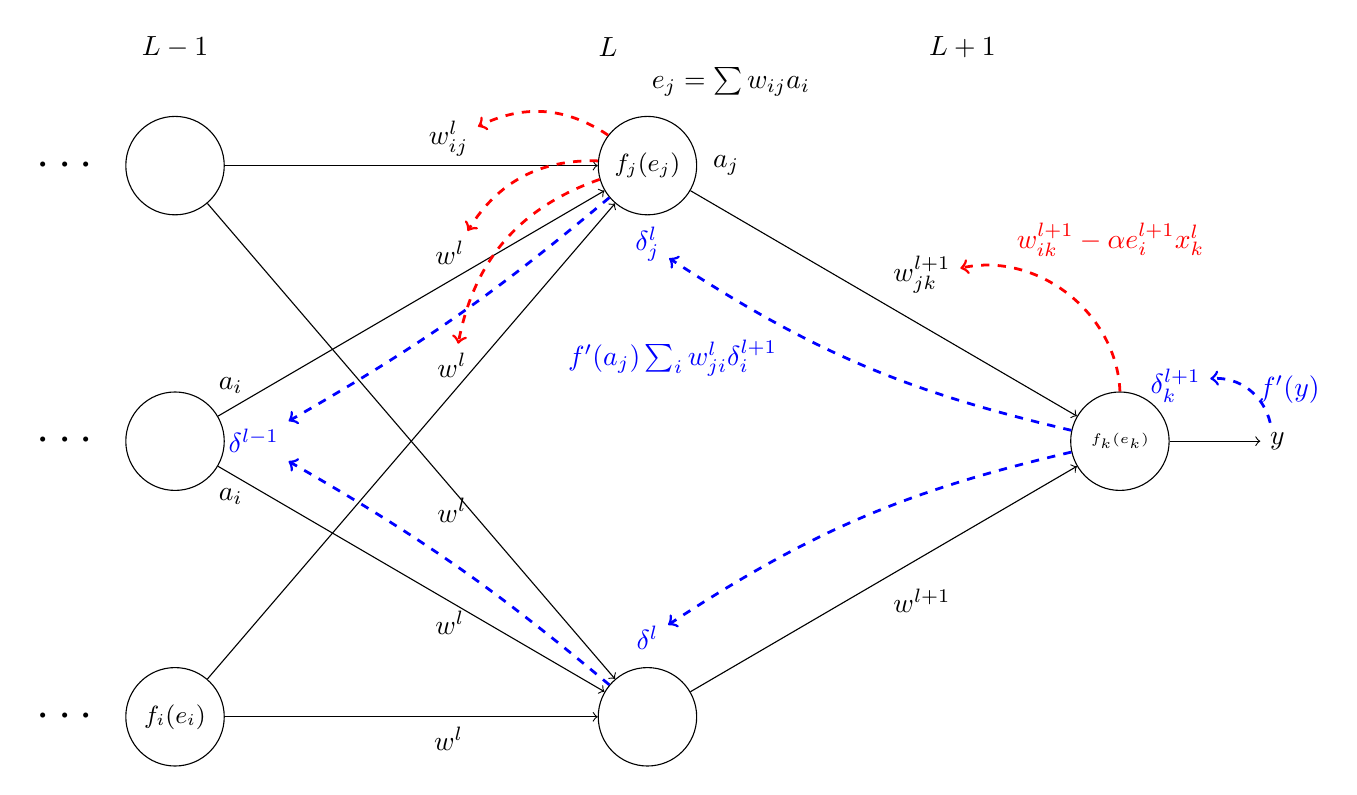
\begin{tikzpicture}

	\tikzstyle{nodo}=[circle, draw, minimum size=1.25cm]
	\tikzstyle{upw}=[dashed, red, ->, line width = 1pt]

	\coordinate (l_0) at (0, 5.0);
	\coordinate (l_1) at (5.5, 5.0);
	\coordinate (l_2) at (10, 5.0);

	\coordinate (f_1_1) at (0, 3.5); % CAPA ENTRADA
	\coordinate (f_1_2) at (0, 0); % CAPA ENTRADA
	\coordinate (f_1_3) at (0, -3.5); % CAPA ENTRADA
	\coordinate (f_2_1) at (6.0, 3.5); % CAPA OCULTA 1
	\coordinate (f_2_2) at (6.0, -3.5); % CAPA OCULTA 1
	\coordinate (f_3_1) at (12, 0); % CAPA SALIDA
	\coordinate (y) at (14, 0); % CAPA SALIDA

	\node[] (l_0) at (l_0) {$L - 1$};
	\node[] (l_1) at (l_1) {$L$};
	\node[] (l_2) at (l_2) {$L + 1$};

	\node[nodo] (f_1_1) at (f_1_1) {}; % CAPA ENTRADA
	\node[nodo] (f_1_2) at (f_1_2) {}; % CAPA ENTRADA
	\node[nodo] (f_1_3) at (f_1_3) {\small $f_i(e_i)$}; % CAPA ENTRADA
	\node[nodo] (f_2_1) at (f_2_1) {\small $f_j(e_j)$}; % CAPA OCULTA 1
	\node[nodo] (f_2_2) at (f_2_2) {}; % CAPA OCULTA 1
	\node[nodo] (f_3_1) at (f_3_1) {\tiny $f_k(e_k)$}; % CAPA SALIDA
	\node[] (y) at (y) {$y$}; % CAPA SALIDA

	\node[left of=f_1_1, node distance=1.4cm] {\LARGE $\cdots$};
	\node[left of=f_1_2, node distance=1.4cm] {\LARGE $\cdots$};
	\node[left of=f_1_3, node distance=1.4cm] {\LARGE $\cdots$};

	\draw[->] (f_1_1) -- node[pos=0.6, above] (w_1_1) {$w^{l}_{ij}$} (f_2_1);
	\draw[->] (f_1_2) -- node[pos=0.6, above] (w_1_2) {$w^{l}_{}$} (f_2_1);
	\draw[->] (f_1_3) -- node[pos=0.6, above] (w_1_3) {$w^{l}_{}$} (f_2_1);
	\draw[->] (f_1_1) node[above right of=f_1_2] {$a_{i}$} -- node[pos=0.6, below] (w_2_1) {$w^{l}_{}$} (f_2_2);
	\draw[->] (f_1_2) node[below right of=f_1_2] {$a_{i}$} -- node[pos=0.6, below] (w_2_2) {$w^{l}_{}$} (f_2_2);
	\draw[->] (f_1_3) -- node[pos=0.6, below] (w_2_3) {$w^{l}_{}$} (f_2_2);
	\draw[->] (f_2_1) node[right of=f_2_1] {$a_{j}$} -- node[pos=0.5, above right] (w_j_k) {$w^{l+1}_{jk}$} (f_3_1);
	\draw[->] (f_2_2) -- node[pos=0.5, below right] {$w^{l+1}$} (f_3_1);
	\draw[->] (f_3_1) -- node[pos=0.5, below right] {$$} (y);

	\node[above right of=f_2_1, node distance=1.5cm] {$e_{j} = \sum w_{ij}a_i$};


	\draw[upw] (f_3_1) to[bend right=50] node[above right, pos=0.8] {$w^{l+1}_{ik} - \alpha e^{l+1}_{i}x^{l}_{k}$} (w_j_k);
	\draw[upw] (f_2_1) to[bend right=30] node[above]{$$} (w_1_1);
	\draw[upw] (f_2_1) to[bend right=30] node[above]{$$} (w_1_2);
	\draw[upw] (f_2_1) to[bend right=30] node[above]{$$} (w_1_3);


	\node[blue, above right of=f_3_1] (e_i) {$\delta^{l+1}_{k}$};
	\node[blue, below of=f_2_1] (e_2_1_i) {$\delta^{l}_{j}$};
	\node[blue, above of=f_2_2] (e_2_2_i) {$\delta^{l}$};
	\node[blue, right of=f_1_2] (e_1_2_i) {$\delta^{l-1}$};

	\draw[upw, blue] (y) to[bend right=40] node[right]{$f'(y)$} (e_i);
	\draw[upw, blue] (f_3_1) to[bend left=10] node[below left, pos=0.7]{$f'(a_{j})\sum_{i}w^{l}_{ji}\delta^{l+1}_{i}$} (e_2_1_i);
	\draw[upw, blue] (f_3_1) to[bend right=10] (e_2_2_i);

	\draw[upw, blue] (f_2_1) to[bend left=5] (e_1_2_i);
	\draw[upw, blue] (f_2_2) to[bend right=5] (e_1_2_i);

\end{tikzpicture}
